\documentclass[12pt,letterpaper]{article}
\usepackage[utf8]{inputenc}
\usepackage{listings, float, xcolor}

%----- Configuración del estilo del documento------%
\usepackage{graphicx, fancyhdr}
\usepackage{enumitem, pifont, hyperref, ulem, tabularx}
\usepackage[left=2cm,right=2cm,top=1.8cm,bottom=2.3cm]{geometry}
\usepackage{hyperref}
\usepackage{lastpage}

%------ Paquetes matemáticos básicos --------%
\usepackage{amsmath, amssymb, amsthm}

\begin{document}

%------ Encabezado -------- %
\begin{center}
\newcommand{\imp}{\rightarrow}
\newcommand{\vp}{\varphi}
  \begin{minipage}{3cm}
    \begin{center}
      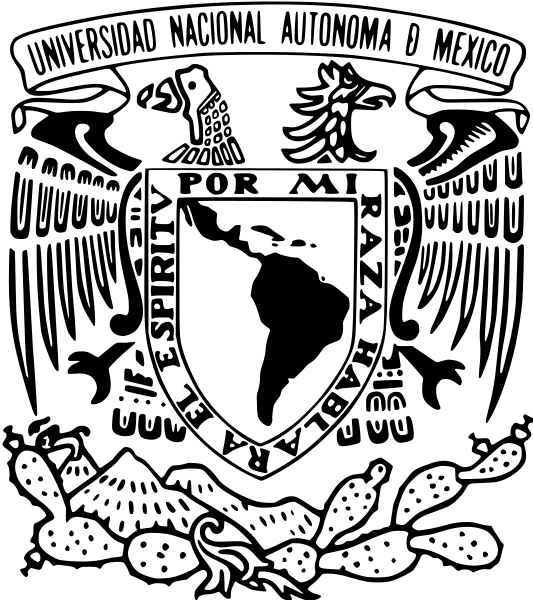
\includegraphics[height=3.4cm]{../unam_logo.png}
    \end{center}
  \end{minipage}\hfill
  \begin{minipage}{10cm}
    \begin{center}
      \textbf{\Large Universidad Nacional Autónoma de México}\\[0.2cm]
      \textbf{\large Facultad de Ciencias}\\[0.2cm]
      \textbf{Organización y Arquitectura de Computadoras 2025-2}\\[0.4cm]
      \textbf{\Large Práctica 06}\\[0.1cm]
      \textbf{Docentes:}\\
      José Galaviz \hspace{1em} Ricardo Pérez \hspace{1em} Ximena Lezama\\[0.3cm]
      \textbf{Autores:}\\
      Fernanda Ramírez Juárez \quad Ianluck Rojo Peña\\[0.3cm]
      \textbf{Fecha de entrega:} Jueves 27 de marzo de 2025
    \end{center}
  \end{minipage}\hfill
  \begin{minipage}{3cm}
    \begin{center}
      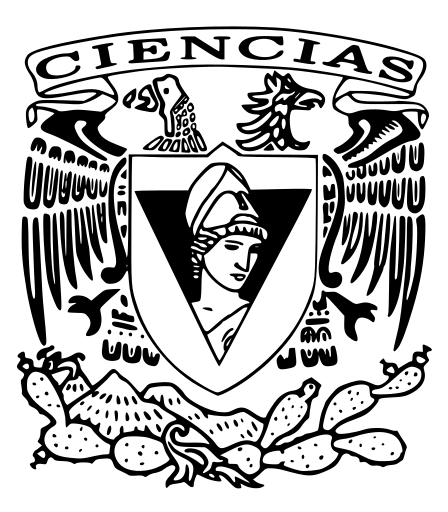
\includegraphics[height=3.4cm]{../fc_logo.png}
    \end{center}
  \end{minipage}
\end{center}

\bigskip
\hrule height 0.1pt
\bigskip

%------ Contenido -------- %
\section*{Preguntas.}

\begin{enumerate}
\item ¿Qué hacen las instrucciones de tipo FR y de tipo FI? Da algunos ejemplos de instrucciones de este tipo y menciona por que están separadas de las otras 3 principales.
  \bigskip
  % -- Respuesta -- %
  
  Las instrucciones de tipo \textbf{FR} \textit{(Floating-Point Register)} y \textbf{FI} \textit{(Floating-Point Immediate)} son aquellas que se encargan de realizar operaciones con números de punto flotante. A diferencia de las instrucciones que trabajan con enteros, estas están diseñadas específicamente para manejar números con partes fraccionarias, lo cual es esencial para cálculos científicos, gráficos y muchas otras aplicaciones.
  
  La diferencia principal entre las instrucciones de tipo \textbf{FR} \textit{(Floating-Point Register)} y \textbf{FI} \textit{(Floating-Point Immediate)} radica en el tipo de operando que utilizan. Las instrucciones FR operan principalmente con valores que se encuentran en los registros de punto flotante y las instrucciones FI operan con un valor inmediato (una constante codificada directamente en la instrucción) y/o realizan transferencias de datos entre la memoria y los registros de punto flotante.\\

  \textbf{Ejemplos de instrucciones FR:}
  
  \begin{itemize}
  \item \texttt{ADD.S \$f2, \$f4, \$f6}:
    Suma el contenido de los registros de punto flotante \$f4 y \$f6, y guarda el resultado en \$f2 (operación de precisión simple).
    
  \item \texttt{MUL.D \$f8, \$f10, \$f12}:
    Multiplica el contenido de los registros de punto flotante \$f10 y \$f12, y guarda el resultado en \$f8 (operación de doble precisión).
    
  \item \texttt{DIV.S \$f14, \$f16, \$f18}:
    Divide el contenido del registro \$f16 entre el de \$f18, y guarda el resultado en \$f14 (precisión simple).
    
  \item \texttt{SQRT.D \$f20, \$f22}:
    Calcula la raíz cuadrada del valor en \$f22 y la guarda en \$f20 (doble precisión).
    
  \item \texttt{C.LT.S \$f24, \$f26}:
    Compara si el valor en \$f24 es menor que el valor en \$f26. El resultado de la comparación se guarda en un registro de condición especial.
  \end{itemize}

  
  \textbf{Ejemplos de instrucciones de tipo FI:}
  \begin{itemize}
  \item \texttt{L.S \$f28, offset(\$rs)}:
    Carga un valor de punto flotante de precisión simple desde la dirección de memoria calculada como \textit{offset} + contenido de \$rs al registro \$f28. Aunque involucra memoria, la carga de un valor de punto flotante se considera dentro de este grupo por su naturaleza de dato.
    
  \item \texttt{S.D \$f30, offset(\$rt)}:
    Almacena el valor de punto flotante de doble precisión del registro \$f30 en la dirección de memoria calculada como \textit{offset} + contenido de \$rt.
  \end{itemize}
  
  Estas instrucciones están separadas de las otras tres principales \textit{(tipo R, tipo I y tipo J)} por lo siguiente:
  
  \begin{itemize}
  \item Los números de punto flotante se representan y manipulan de manera distinta, lo que crea la necesidad de tener hardware especializado dentro del procesador para realizar las operaciones de manera eficiente.
  \item Las arquitecturas tienen un conjunto de registros separado (como los registros \$f en MIPS) para almacenar valores de punto flotante. Esto permite optimizar el diseño del hardware para cada tipo de dato.
  \item Las operaciones de punto flotante son más complejas a nivel de hardware que las operaciones enteras básicas. Separarlas permite que la unidad de enteros se mantenga más simple y rápida para las tareas que no requieren aritmética de punto flotante.
  \item Las instrucciones de punto flotante tienen formatos diferentes para acomodar los operandos de punto flotante y los códigos de operación específicos para estas operaciones.
  \end{itemize}
  \bigskip
  
\item ¿Qué es la Portabilidad de Arquitecturas \textbf{(Cross-Architecture Porting)}?
  \bigskip
  % -- Respuesta -- % 

  La Portabilidad de Arquitecturas \textbf{(Cross-Architecture Porting)} se refiere a la capacidad de un programa o software para una arquitectura de hardware de ser ejecutado en otra arquitectura de hardware diferente con una mínima o ninguna modificación en su código fuente.

  Lograr una portabilidad completa a nivel de código ensamblador es extremadamente difícil, ya que el lenguaje ensamblador es naturalmente específico de una arquitectura en particular; además cada arquitectura tiene su propio conjunto de instrucciones, organización de registros, modos de direccionamiento y convenciones de llamada.
  
  En la práctica, la portabilidad de arquitecturas generalmente se logra escribiendo software en lenguajes de alto nivel \textbf{(como C, C++, Java o Python)} que son independientes de la arquitectura base; este código fuente se compila para la arquitectura de destino utilizando un compilador específico para esa arquitectura. El compilador se encarga de traducir el código de alto nivel a las instrucciones de ensamblador nativas de la arquitectura objetivo.

  Por lo tanto, cuando hablamos de portabilidad de arquitecturas, rara vez se refiere a tomar un programa escrito directamente en ensamblador para una arquitectura y ejecutarlo sin cambios en otra. Más bien implica diseñar sistemas y escribir código de manera que pueda ser adaptado y recompilado fácilmente para diferentes plataformas de hardware.
  \bigskip
  
\item Menciona 5 llamadas a sistema \textit{(syscall)} que puedes usar en MIPS. Menciona su código de instrucción y qué es lo que hace.
  \bigskip
  % -- Respuesta -- % 

  \begin{table}[H]
    \centering
    \resizebox{\textwidth}{!}{ % Ajusta la tabla al ancho del documento
    \begin{tabular}{| m{3cm} | m{4cm} | m{3cm} | m{4cm} | m{3cm} |}
        \hline
        \textbf{Servicio} & \textbf{Operación} & \textbf{Código en \$v0} & \textbf{Argumentos} & \textbf{Resultado} \\ \hline
        \textbf{print\_int}    & Imprime un número entero (32 bits) & 1 & \$a0 = entero a imprimir & Ninguno \\ \hline
        \textbf{print\_string} & Imprime una cadena de caracteres con terminación null & 4  & \$a0 = dirección en memoria de la cadena a imprimir & Ninguno \\ \hline
        \textbf{print\_char}   & Imprime un carácter & 11 & \$a0 = carácter a imprimir & Ninguno \\ \hline
        \textbf{read\_int}     & Lee el número entero ingresado por el usuario & 5  & Ninguno & Regresa el número en \$v0 \\ \hline
        \textbf{read\_string}  & Igual que la función \textit{fgets()} de la biblioteca estándar en C & 8  & \$a0 = dirección en memoria del buffer de entrada de la cadena, \$a1 = longitud del buffer de la cadena (n) & Ninguno \\ \hline
    \end{tabular}
    }
\end{table}
  
  \bigskip

\item ¿Cuáles son los 3 tipos principales de instrucciones? Menciona que comportamiento tiene cada tipo de instrucción.
  \bigskip
  % -- Respuesta -- %
  \begin{enumerate}[label=\arabic*)]
  \item \textbf{Operaciones de tipo R (Register-type):}\\
    Las instrucciones de tipo R se usan cuando todos los valores involucrados en la operación se encuentran en los registros del procesador. Estas instrucciones realizan operaciones aritméticas y lógicas sin acceso a memoria.
    
    El formato general de una instrucción tipo R es:
    \[
    \texttt{OP \ rd, rs, rt}
    \]
    Donde:
    \begin{itemize}
    \item \textbf{rs} y \textbf{rt} son los registros fuente.
    \item \textbf{rd} es el registro destino donde se almacenará el resultado.
    \end{itemize}
    
    Aquí un ejemplo de la instrucción \texttt{add}:
    \begin{verbatim}
    add $t0, $t1, $t2   # $t0 = $t1 + $t2
    \end{verbatim}

  \item \textbf{Operaciones de tipo I (Immediate-type):}\\
    Las instrucciones de tipo I se utilizan cuando es necesario operar con un valor inmediato (constante) y un registro. Los valores inmediatos en MIPS tienen un máximo de 16 bits, por lo que números más grandes no pueden ser manejados directamente con instrucciones inmediatas.
    
    El formato general de una instrucción tipo I es:
    \[
    \texttt{OP \ rt, IMM(rs)}
    \]
    Donde:
    \begin{itemize}
    \item \textbf{rt} es el registro donde se almacenará el resultado.
    \item \textbf{IMM} es el valor inmediato.
    \item \textbf{rs} es el registro base (en operaciones con memoria).
    \end{itemize}
    
    Ejemplo de la instrucción \texttt{addi}:
    \begin{verbatim}
    addi $t0, $t1, 10   # $t0 = $t1 + 10
    \end{verbatim}

  \item \textbf{Operaciones de tipo J (Jump-type):}\\
    Las instrucciones de tipo J son utilizadas para realizar saltos a direcciones específicas en la memoria. Estas instrucciones tienen mayor capacidad para manejar valores inmediatos, ya que trabajan con direcciones de memoria más grandes.
    
    El formato general de una instrucción tipo J es:
    \[
    \texttt{OP \ LABEL}
    \]
    Donde:
    \begin{itemize}
    \item \textbf{LABEL} es la dirección de memoria o etiqueta a donde se debe saltar.
    \end{itemize}

    Ejemplo de la instrucción \texttt{j}:
    \begin{verbatim}
    j etiqueta  # Salta a la dirección de memoria etiquetada
    \end{verbatim}
  \end{enumerate}
  \bigskip
  
\end{enumerate}
\end{document}
